%http://www.latexstudio.net/archives/1713.html
%画未知解析式曲线切线
%!TEX program = pdflatex
\documentclass{article}
\usepackage{tikz,pgfplots}
\pgfplotsset{compat=1.8}
\usepackage{mathpazo}

\usetikzlibrary{arrows,calc}
\usetikzlibrary{decorations.markings}

%使用 TikZ 绘制已知表达式曲线的切线
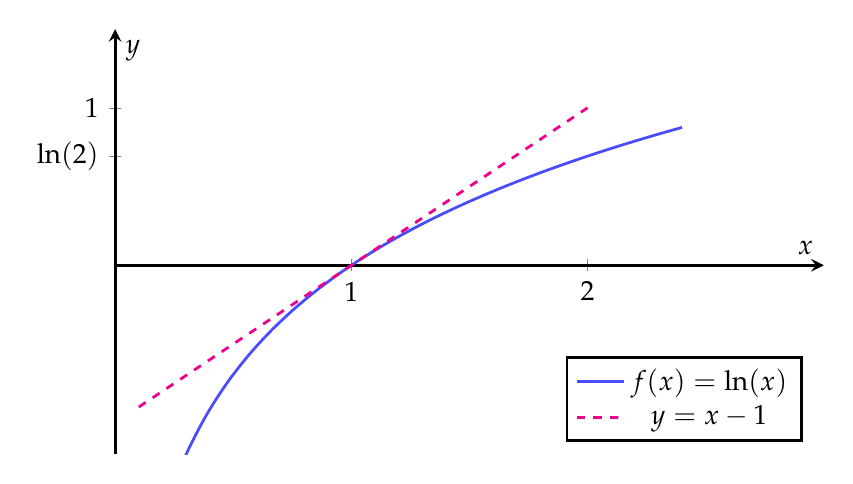
\begin{tikzpicture}
  \begin{axis}[
      legend pos=south east,
      y=2cm, x=3cm,
      xlabel={$x$}, ylabel={$y$},
      xmin=0, xmax=3,
      ymin=-1.2, ymax=1.5,
      xtick={0,1,2}, ytick={0,0.6931471806,1},
      xticklabels={0,1,2}, yticklabels={0, $\ln(2)$,1},
      line width=1pt,
      axis lines=center,
      ]
      \addplot [smooth, domain=0.2:2.4, blue!70] {ln(x)};
      \addlegendentry{$f(x) = \ln(x)$}
      \addplot [smooth, domain=0.1:2.0, magenta, dashed] {x-1};
      \addlegendentry{$y = x - 1$}
  \end{axis}
\end{tikzpicture}
\par
% 使用 TikZ 绘制未知表达式曲线的切线一、使用 markings 实现对点的定位
\begin{tikzpicture}[
   tangent/.style={
       decoration={
           markings,% switch on markings
           mark=
               at position #1
               with
               {
                   \coordinate (tangent point-\pgfkeysvalueof{/pgf/decoration/mark info/sequence number}) at (0pt,0pt);
                   \coordinate (tangent unit vector-\pgfkeysvalueof{/pgf/decoration/mark info/sequence number}) at (1,0pt);
                   \coordinate (tangent orthogonal unit vector-\pgfkeysvalueof{/pgf/decoration/mark info/sequence number}) at (0pt,1);
               }
         },
         postaction=decorate
       },
     use tangent/.style={
         shift=(tangent point-#1),
         x=(tangent unit vector-#1),
         y=(tangent orthogonal unit vector-#1)
     },
     use tangent/.default=1
  ]
  \draw [<->,>=stealth'] (0,5) node [label = left:{$f(x)$}]{} -- (0,0) -- (8.5,0) node[label = below:{$x$}]{};
  \draw [
     tangent=0.4,
     tangent=0.56,
  ] (0.1,0.1)
     to [out=20,in=120] (4,2.5)
     to [out=-60, in=110] (8,3);
  \draw [blue, thick, use tangent] (-3,0) -- (3,0);
  \draw [orange, thick, use tangent=2] (-2,0) -- (2,0) (0,0) -- (0,1);
\end{tikzpicture}
\par
% 使用 TikZ 绘制未知表达式曲线的切线二、使用 node 作为初始点新建局部的坐标系
\begin{tikzpicture}[allow upside down,scale=0.7]
  \draw [<->,>=stealth'] (0,5.5) node [label = left:{$f(x)$}]{} -- (0,0) -- (9,0) node[label = below:{$x$}]{};

   % 将路径画出来,然后选择切点位置为 0.5
  \draw[black,line width=1pt] (0,0) .. controls (5,1) and  (6,2) .. (8,5)
        node[sloped,inner sep=0cm,above,pos=0.5,
        anchor=south west,
        minimum height=(10.5)*0.3cm,minimum width=(10.5)*.3cm](N){};
   % 绕 N 建立局部的参照点
  \path (N.south west)%
             edge[-stealth',blue] node[left] {$\vec{ n}$} (N.north west)
             edge[-stealth',blue] node[above] {$\vec{ t}$} (N.south east);
  \path [draw,magenta,thick,dashed](N.south east)--(N.south west) -- ($(N.south west)!1!180:(N.south east)$);

   % 灰色线为点 N 所在垂直的直角坐标系
  \draw[-stealth',gray]  (N.south west)  --%
        node[below] {$\vec{t_a}$} (N.south west -| N.south east);
  \draw[-stealth',gray]  (N.south west)  --%
        node[right] {$\vec{t_o}$} (N.south west |- N.south east);
\end{tikzpicture}
\par
\end{document}
